\documentclass[12pt]{article}

% Packages
\usepackage{graphicx}
\usepackage{subcaption}
\usepackage{amsmath, amssymb, amsfonts}
\usepackage{siunitx}
\usepackage{array}
\usepackage[T1]{fontenc}
\usepackage{textcase}
\usepackage{caption}
\usepackage{fancyhdr}
\usepackage{lettrine}
\usepackage{geometry}
\usepackage{caption}
\usepackage{bm}
\usepackage{float}
\usepackage{enumitem}
\usepackage[backend=biber,style=ieee]{biblatex}
\usepackage{titlesec}
\usepackage[hidelinks]{hyperref}

% Geometry and Paths
\geometry{letterpaper, margin=1in}
\graphicspath{{../../images/}}

% Header and Footer
\makeatletter
\newcommand{\papertitle}{Vision Vs. LiDAR/Radar Fusion in ADS}

% re-define \sectionmark so that only top-level \section updates \leftmark
\renewcommand{\sectionmark}[1]{%
  \markboth{\Roman{section}. #1}{}%
}
% Header and Footer
\pagestyle{fancy}
\fancyhf{}
\fancyhead[R]{\scriptsize\leftmark{} – \thepage}
\fancyfoot[R]{\scriptsize\MakeUppercase{\papertitle}}
\setlength{\headheight}{15pt}
\makeatother

% Bibliography
\addbibresource{sources.bib}

\titleformat{\section}
  {\centering\large\scshape}               % shape
  {\Roman{section}.}                        % label
  {1em}                                     % sep
  {}                                        % before-code
\titlespacing*{\section}{0pt}{1.5em}{1em}

\titleformat{name=\section,numberless}
  {\centering\large\scshape}{}{1em}{}
\titlespacing*{name=\section,numberless}{0pt}{1.5em}{1em}

\titleformat{\subsection}[block]
  {\itshape}                               % italic
  {\Alph{subsection}.}                     % label
  {1em}                                     % sep
  {}                                        % before-code
\titlespacing*{\subsection}{0pt}{1em}{0.5em}

% 3) Tertiary (1), 2), …) — block, no colon
\titleformat{\subsubsection}[block]
  {\itshape}                          % italic shape
  {\arabic{subsubsection})}           % label “1)”
  {1em}                                % sep between label and title
  {}                                   % before-code (empty)
\titlespacing{\subsubsection}{1em}{0.75em}{0.5em}

% 4) Quaternary (a), b), …) — block, no colon
\titleformat{\paragraph}[block]
  {\itshape}                          % italic shape
  {\alph{paragraph})}                 % label “a)”
  {1em}                                % sep
  {}                                   % before-code
\titlespacing{\paragraph}{2em}{0.75em}{0.5em}

% CAPTIONS
\captionsetup{font=footnotesize}
\captionsetup[figure]{%
  labelformat=simple,
  name=Fig.,
  labelsep=period,
  justification=centering,
  singlelinecheck=false
}
\renewcommand{\thetable}{\Roman{table}}
\DeclareCaptionLabelFormat{dropcapsmall}{%
  {\small T}{\footnotesize\scshape able}~#2%
}
\captionsetup[table]{%
  labelformat=dropcapsmall,
  labelsep=newline,
  justification=centering,
  singlelinecheck=false
}
% Title Page
\title{\bfseries\LARGE Vision Vs. LiDAR/Radar Fusion in Autonomous Driving Systems}
\author{Arturo Salinas-Aguayo}

\begin{document}

\begin{titlepage}
    \centering
    \vspace*{3cm}
    {\Large \textsc{Vision Vs. LiDAR/Radar Fusion in Autonomous Driving
		Systems}}\\
		Arturo Salinas-Aguayo, \textit{BS Computer Engineering, Class of 2027}\\
		\today\\
    \vspace{1.5cm}
    ECE 4900W: Communicating Engineering Solutions in a Societal Context\\
    Dr. Shengli Zhou, SEC040-1255\\
    Department of Electrical and Computer Engineering\\
    \vfill
    
\includegraphics[scale=0.1]{uconnlogo}\\[1em]
    University of Connecticut College of Engineering\\
    \small\tiny{Coded in \LaTeX} \\
    \vspace{1cm}
\end{titlepage}

\tableofcontents
\newpage

\section*{Abstract}
\addcontentsline{toc}{section}{Abstract}

This paper evaluates the viability of vision-primary perception systems in
autonomous driving, focusing on scalability, efficiency, and environmental
resilience. Traditional sensor-fusion architectures based on LiDAR and radar
offer high-fidelity spatial mapping but suffer from substantial power
consumption, mechanical complexity, and high unit costs, which challenge
real-time deployment and mass-market feasibility. Advances in neural
perception—particularly transformer-based models and tokenized camera
inputs—have enabled camera-only systems to approximate LiDAR-level 3D detection
accuracy while operating at a fraction of the computational cost. Benchmark
evaluations reveal that vision systems achieve depth estimation errors below
three percent and perform within five percent of LiDAR/Radar fusion baselines in object detection.
Critically, performance gaps in adverse conditions such as fog or night driving are recoverable through the selective integration of millimeter-wave radar. This radar-augmented fallback restores over 80 percent of degraded performance with minimal latency or energy impact. The study advocates for a simplified, vision-first architecture complemented by radar only in edge cases. This paradigm enhances scalability, reduces deployment overhead, and aligns with biologically plausible sensing strategies. LiDAR remains useful for simulation and benchmarking but is unnecessary for live inference.

\textbf{Index Terms—Adverse weather robustness, autonomous vehicles, deep
	learning, depth estimation, energy efficiency, Light Detection and Ranging
(LiDAR), Radar, sensor fusion, Transformer networks, vision-based perception.}
\newpage

\section{Introduction}

As vehicles become more technologically advanced, the demand for autonomous
capabilities continues to rise. Features such as lane keeping, adaptive cruise
control, and highway autopilot—collectively known as autonomous driving systems (ADS)—form the early building blocks of full self-driving stacks. Industry leaders now face a critical decision: how should vehicles perceive the road ahead?

Historically, high-end systems such as Waymo and Cruise relied on Light Detection and Ranging (LiDAR) and radar to construct dense, 3D maps of their surroundings. These sensors offer precise geometry and reliable velocity estimation, but impose high hardware cost, weight, and power draw. Moreover, integrating data from multiple sensors increases architectural complexity and susceptibility to calibration drift.

In contrast, Tesla, Comma.ai, and others have adopted a vision-first approach. These systems rely on arrays of low-cost cameras and train deep neural networks—often transformers—on large-scale driving datasets. Rather than reconstruct explicit 3D geometry, these models learn to infer structure and intent directly from pixels.

The debate between fusion-heavy and camera-only stacks now defines the frontier of ADS design. While LiDAR remains dominant in academia, vision-based approaches have rapidly improved in real-world performance and outpace fusion in scalability. From a societal perspective, the ability to deliver autonomy without costly sensors is especially important in emerging markets, where a single LiDAR unit may cost more than an entire car.

This report compares the two paradigms by analyzing their theoretical foundations, energy profiles, data fidelity, and robustness under real-world driving conditions.

\section{Technology Description}

\subsection{SAE Levels of Automation}

The Society of Automotive Engineers (SAE) J3016 standard defines six levels of
vehicle automation \cite{SAEJ3016_2021}. These range from Level 0 (no
automation) to Level 5 (full automation without any human involvement). The full
description of each level is given in Table~\ref{tab:sae}.

\begin{table}[H]
  \centering
  \caption{SAE J3016 Levels of Driving Automation}
  \label{tab:sae}
  \begin{tabular}{|p{5.5cm}|p{9.5cm}|}
    \hline
    \textbf{Level} & \textbf{Description} \\
    \hline
    Level 0 – No Automation & The human driver is responsible for all tasks; the system may provide basic warnings. \\
    \hline
    Level 1 – Driver Assistance & The system assists with either steering or speed, but not both; driver must stay engaged. \\
    \hline
    Level 2 – Partial Automation & The system can manage both speed and steering, but human oversight is still mandatory. \\
    \hline
    Level 3 – Conditional Automation & The vehicle handles all driving in specific scenarios; the driver must intervene when requested. \\
    \hline
    Level 4 – High Automation & No driver input is required in controlled conditions (e.g., geofenced urban areas). \\
    \hline
    Level 5 – Full Automation & The vehicle is capable of full self-driving in all conditions without human input. \\
    \hline
  \end{tabular}
\end{table}

Currently, most ADS operate at Level 2, which is very much like being a
driver's ed instructor sitting at secondary controls while a 15-year-old is
operating the vehicle, ready to take control at any given moment. Level 5 is
ideally like sitting in a train car, with
absolutely no attention needed from the driver. This frees the driver to work on
other important tasks such as grading papers, concentrating on a new idea, or
taking some real downtime at the end of a stressful day.

\subsection{LiDAR: Time-of-Flight (ToF) Principles}

LiDAR estimates object distance using time-of-flight (ToF) measurements, where a light pulse is emitted and its return time is measured. Several ToF techniques are in use:

\subsubsection{Pulsed ToF:}
Pulsed TOF techniques are the simplest of the three cases in which distance is
determined by multiplying the speed of light in a medium by the time a light
pulse takes to travel the distance to the target:
\begin{equation}
R_{\text{pulse}} = \frac{c}{2} t_{\text{oF}},
\label{eq:tof_pulse}
\end{equation}
where $R_{oF}$ is the distance the light ray travels, $c$ is the speed of
light in free space, and $t_{oF}$ is the time it takes for the pulse of energy
to travel from its emitter to the observed object and then back to the receiver.
This high-power method provides centimeter accuracy. This method is shown in
Figure~\ref{fig:pulse}.
\begin{figure}[H]
	\centering
	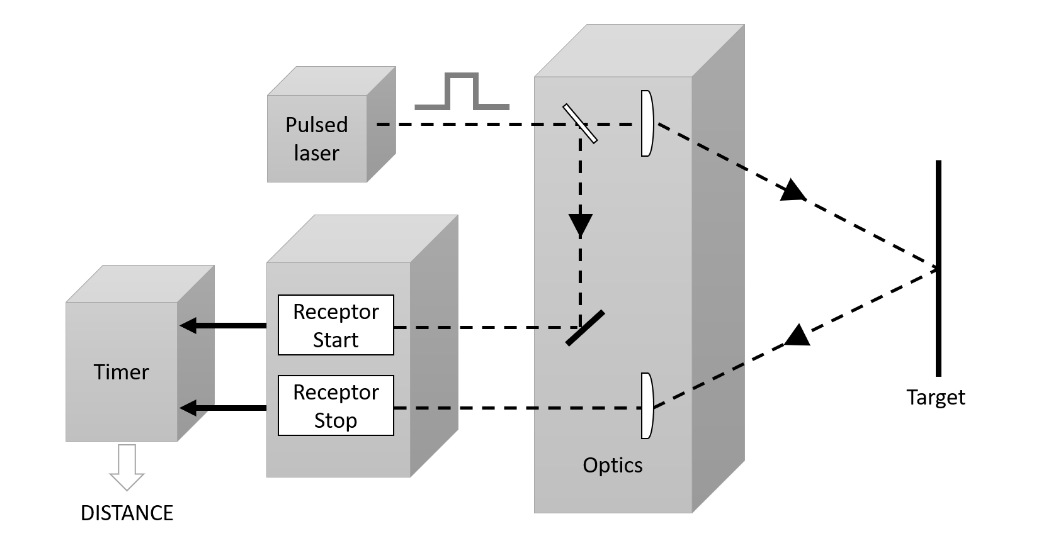
\includegraphics[width=0.6\textwidth]{lidar.png}
	\caption{The Pulsed Approach to Determining Object Distance \cite{2019Royo}}
	\label{fig:pulse}
\end{figure}


\subsubsection{AMCW (Amplitude-Modulated Continuous Wave):}
The AMCW approach modulates the intensity of a continuous lightwave instead of
laser pulsing as utilized in Eqn.~\ref{eq:tof_pulse}. This method utilizes the
corresponding shift in phase in the received signal to calculate the distance to
the object, $R$:
\begin{equation}
R = \frac{c}{2} \cdot \frac{\Delta\Phi}{2\pi f_M},
\label{eq:amcw}
\end{equation}
where \( \Delta\Phi \) is the phase shift, $c$ is the speed of light in free
space, and \( f_M \) is the modulation
frequency \cite{2019Royo}. It's simplified principles are shown in
Figure~\ref{fig:amcw}.
\begin{figure}[H]
	\centering
	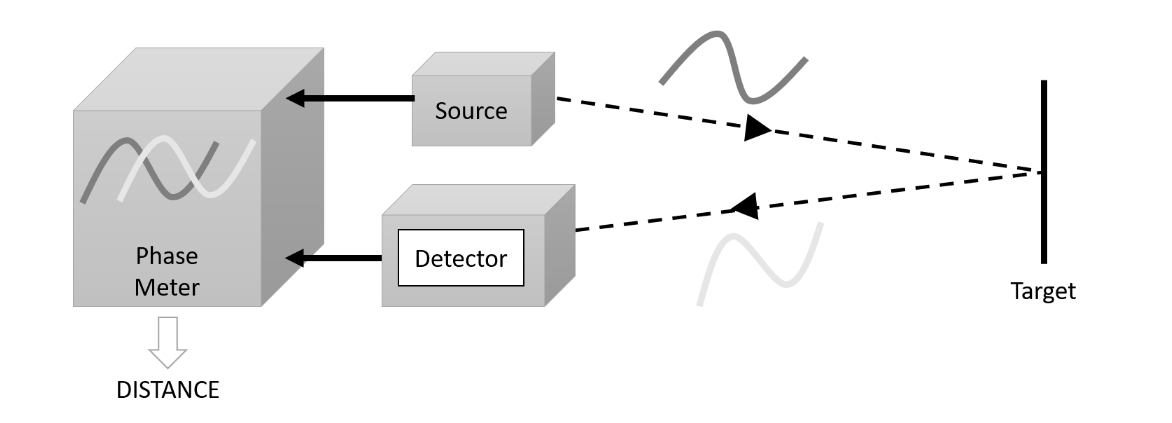
\includegraphics[width=0.6\textwidth]{amcw}
	\caption{Measuring Distance by Phase Difference \cite{2019Royo}}
	\label{fig:amcw}
\end{figure}
\subsubsection{FMCW (Frequency-Modulated Continuous Wave):}
This final method involves a modulating the power applied to the source
\cite{petermannopto}. The signal returned is mixed with the source signal,
creating a beat frequency that is a measure of the probed distance, $R$:
\begin{equation}
R = f_r\frac{c T}{2B},
\label{eq:fmcw}
\end{equation}
where \( f_r \) is the beat frequency, \( T \) the period of the ramp, $c$ is
the speed of light in free space, and \( B \)
the bandwidth of the frequency sweep \cite{2019Royo}. The main parameters are
shown in Figure~\ref{fig:fmcw}.
\begin{figure}[H]
	\centering
	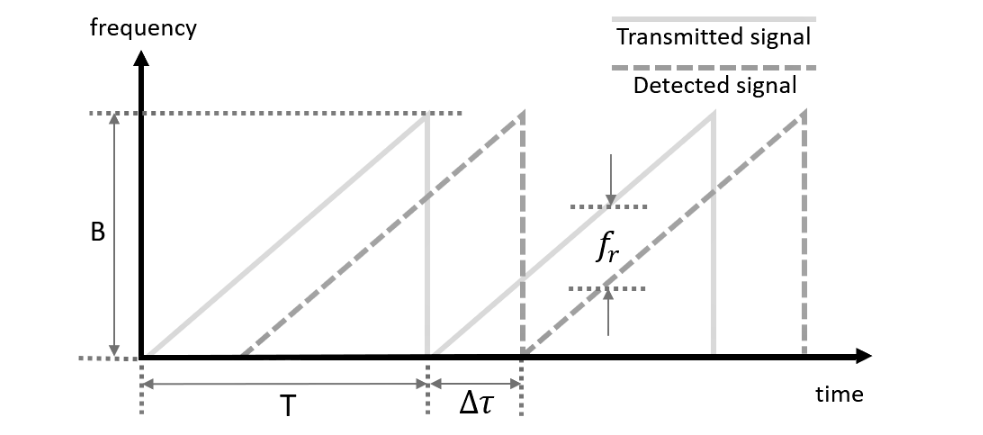
\includegraphics[width=0.6\textwidth]{fmcw}
	\caption{Measuring Distance by Frequency Modulation \cite{2019Royo}}
	\label{fig:fmcw}
\end{figure}
This method is fundamentally different as there is additional processing
overhead done in the Fourier domain rather than in the time or complex domain
for the pulsed and AMCW approach respectively. This ultimately allows precision
to much higher precision \cite{petermannopto}.

\subsubsection{Voxelization:}
What results from the utilization of these methods is a ``point cloud" which
corresponds to the distances the objects are away from the transmitter. The
interpretation of these distances into 3D object boxes is a process called
Voxelization. The high level process of breaking down point clouds into voxels and
interpreting them is shown in Figure~\ref{fig:voxelization}.
\begin{figure}[H]
	\centering
	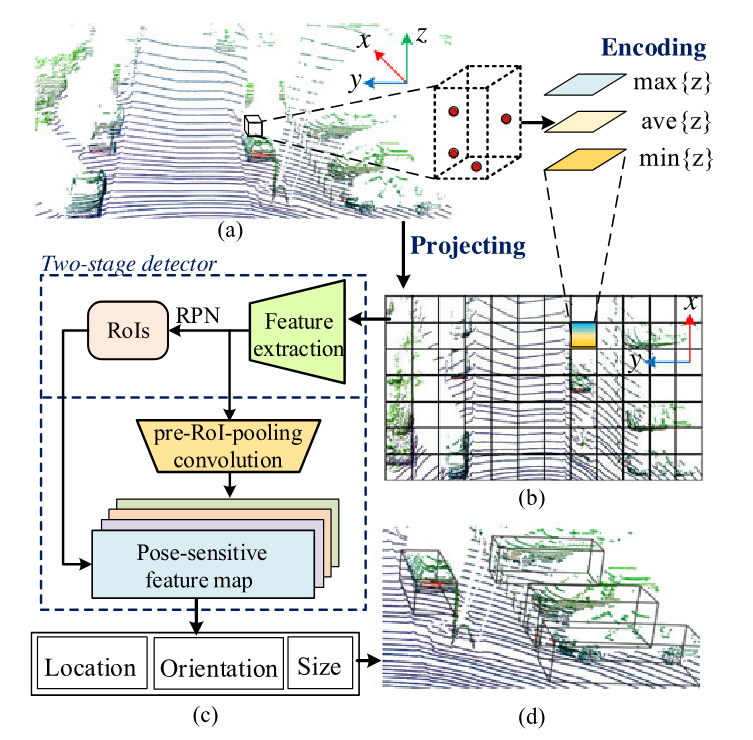
\includegraphics[width=0.6\textwidth]{voxelization.png}
	\caption{The combining of the point cloud forms an image where (a) is the
	interpreted collection of point clouds inferred by the distance calculation in the sensor, (b) is the
segmentation of this set of distances into a grid to create a 'set of sets' of
different points, (c) is the transformer pipeline which leads to object
identification, and (d) is the outcome with identified objects boxed
\autocite{RT3D}.}

	\label{fig:voxelization}
\end{figure}

\subsection{Radar: Doppler and Velocity Estimation}

The Doppler effect is the change in frequency or wavelength of a wave for an
observer or sensor, who is moving relative to the wave source. Radar calculates velocity $v$, via Doppler frequency shift:

\begin{equation}
v = \frac{f_D \lambda}{2},
\label{eq:radar_doppler}
\end{equation}
where \( f_D \) is the Doppler shift and \( \lambda \) is the radar wavelength
\cite{Han2023FourDRadarSurvey}. Radar’s all-weather capability makes it ideal
for fallback use. Figure~\ref{fig:doppler} shows the Doppler effect as it
pertains to humans, a useful tool in understanding how this phenomena can be
applied to this.

\begin{figure}[H]
	\centering
	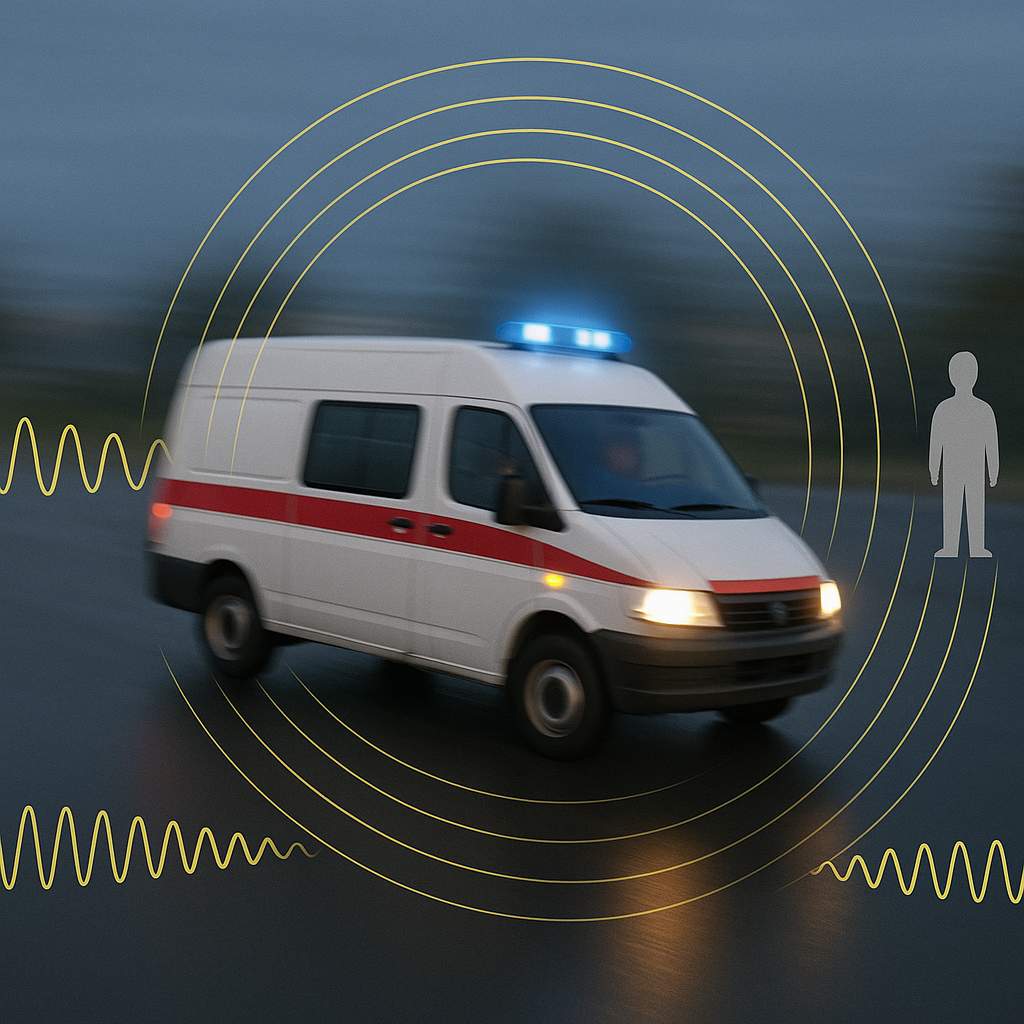
\includegraphics[width=0.4\textwidth]{doppler}
	\caption{The classic Doppler example showing an ambulance emitting sound. An
	observer, from whom the ambulance leaving from will receive fewer pressure and
will hear a deeper note, while an observer from whom the ambulance is
approaching will receive higher pressure fluctuations and hear a higher note.}
	\label{fig:doppler}
\end{figure}
\subsection{Sensor Fusion and Noise Correlation}

Noise is a deviation of the response to the ideal signal and manifests itself
differently depending on the type of sensor in phenomena such as temperature,
EMF, or visual interference (weather). Noise in sensor fusion is modeled as:
\begin{equation}
\sigma_{D_f}^2 = \sum_{i=1}^{n} w_i^2\,\sigma_{D_i}^2 + 2\sum_{i<j} w_i
w_j\,\rho_{ij}\,\sigma_{D_i}\sigma_{D_j},
\label{eq:noise}
\end{equation}

where \( w_i \) are weights, \( \sigma_{D_i} \) are variances, and \( \rho_{ij}
\) are sensor correlations \cite{Rana2023PerceptionSystems}.

\subsection{Vision-Primary Perception Stack}

\subsubsection{System Architecture:}

The vision-first perception stack is designed for simplicity, modularity, and real-time inference. It consists of three core stages:

\begin{enumerate}[label=\alph*)]
  \item Image Tokenization – converts camera frames into a semantically rich, compressed token representation using a learned encoder.
  \item Transformer-Based Planning – autoregressively predicts future trajectory
		tokens from visual context using a transformer model. This is the key to
		making a completely generalizable model.
  \item Control Decoding – transforms predicted spatial tokens into low-level vehicle commands for actuation.
\end{enumerate}

This pipeline emulates language models for sequential prediction and supports real-time operation on embedded platforms \autocite{goff2025learningdriveworldmodel}.

\subsubsection{Token-Based Image Compression:}

Each frame, typically $128 \times 256$ pixels, is passed through a VQGAN encoder
that produces up to 512 discrete tokens per image. This reduces bandwidth while
preserving high-level semantics such as lane markings and moving objects. The
process of encoding these images into tokens is shown in
Figure~\ref{fig:tokenizer}.

\begin{figure}[H]
    \centering
    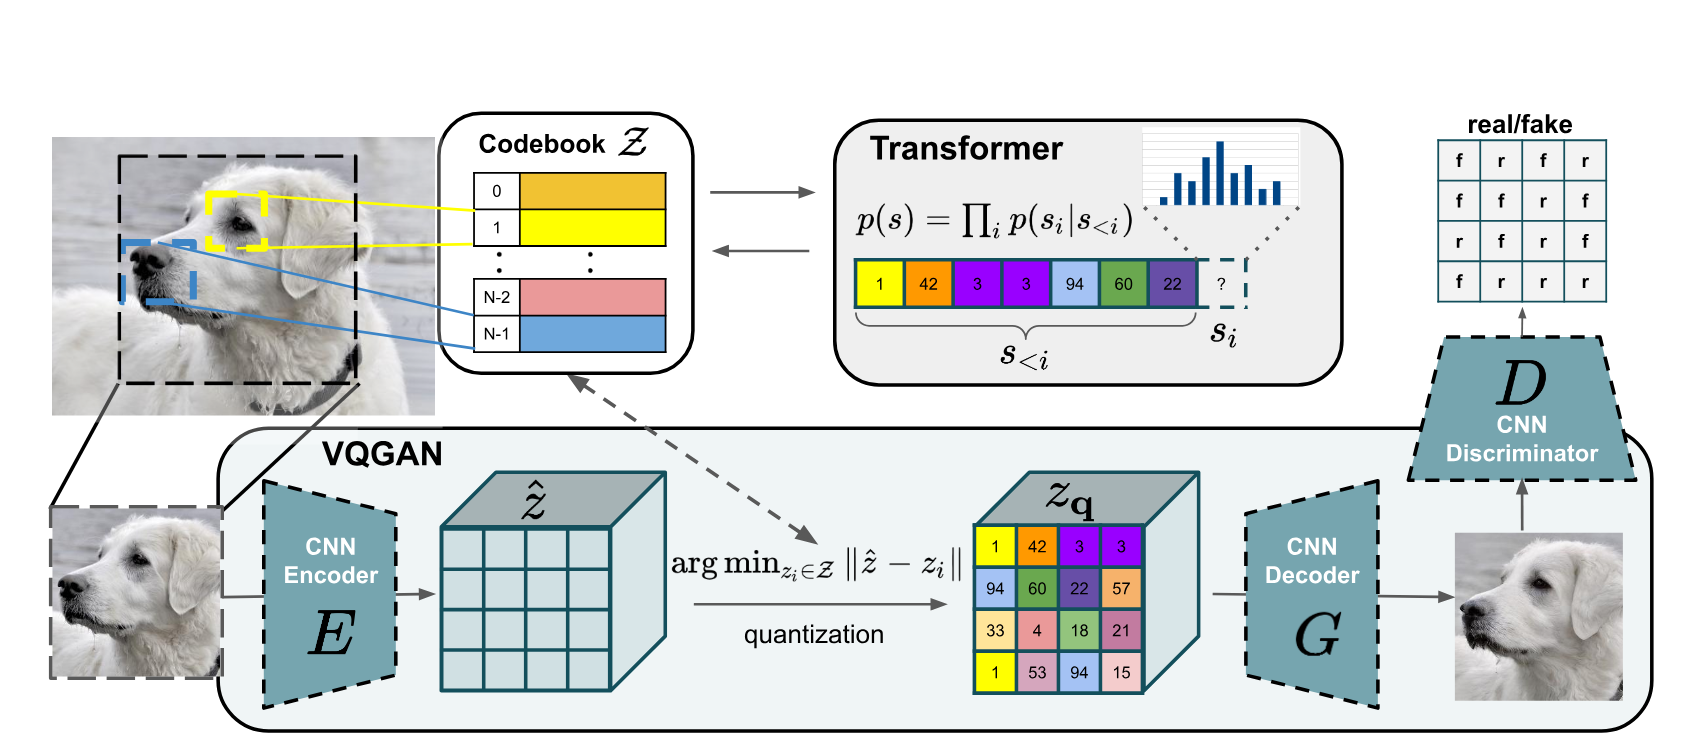
\includegraphics[width=0.8\textwidth]{architecture}
    \caption{Vision-based pipeline with VQGAN tokenization and transformer rollout \autocite{Esser2021TamingTransformersHighResolutionImage}.}
    \label{fig:tokenizer}
\end{figure}

This compact form accelerates inference and reduces power draw without sacrificing depth accuracy \autocite{Chen2024EndToEndAD}.

\subsubsection{Autoregressive Planning with Transformers}
Much like how an LLM can predict the next word in a string through tokenization,
a transformer can predict a variety of outcomes in a driving model from a static
image that is tokenized. The token sequence is processed by a decoder-only
transformer, which predicts the next spatial token at each step. This
architecture parallels natural language processing and enables generalization to
unseen traffic scenarios \cite{drivingsim}. The modern transformer architecture
employed, shown in Figure~\ref{fig:transformer}, is taken from one of the most
important works in recent AI advancement, ``Attention is All You Need"
\cite{vaswani2023attentionneed}.
\begin{figure}[H]
    \centering
    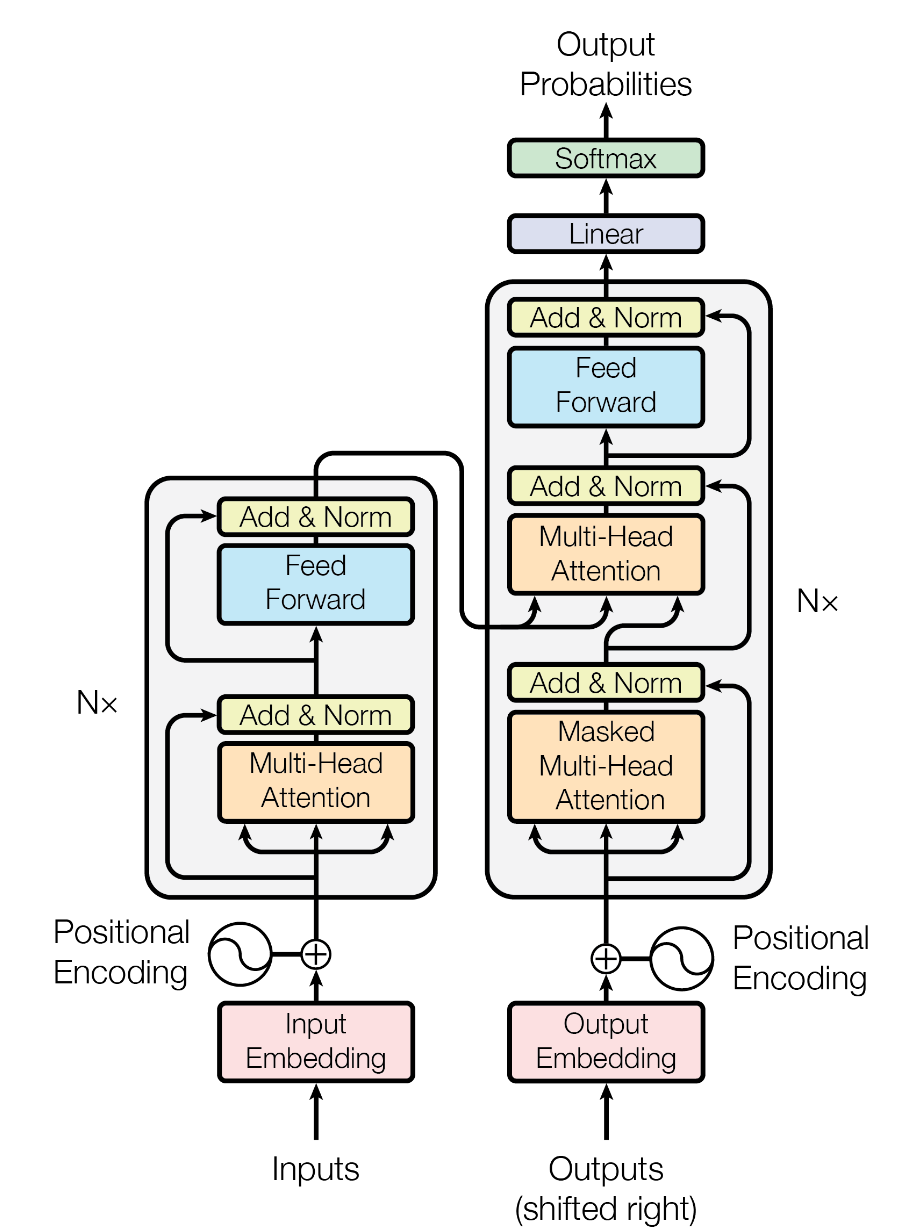
\includegraphics[width=0.5\textwidth]{architecture2}
    \caption{Transformer model for sequence prediction from visual tokens \autocite{vaswani2023attentionneed}.}
    \label{fig:transformer}
\end{figure}

The transformer is trained using imitation learning on datasets like commaVQ and
can be fine-tuned using reinforcement learning for policy robustness
\autocite{drivingsim}. This way, the training data need not have to contain
every situation imaginable, as the process itself will be able to infer all
possible world conditions \cite{goff2025learningdriveworldmodel}. Once all of
these policies are applied and processing is applied, the details in
Figure~\ref{fig:visionpipe} can be inferred.

\begin{figure}[H]
	\centering
	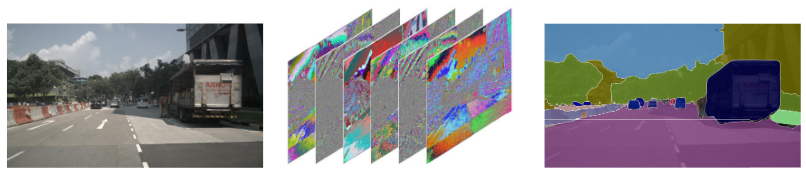
\includegraphics[width=0.9\textwidth]{masking}
	\caption{The Vision Pipeline shows the original camera image, the feature map,
	and the image mask \cite{wang2024}.}
	\label{fig:visionpipe}
\end{figure}

\subsection{LiDAR/Radar Fusion-Based Architecture}

\subsubsection{Pipeline Overview:}

Legacy ADS stacks rely on multi-modal fusion to mitigate sensor weaknesses. A typical LiDAR/radar pipeline includes:

\begin{enumerate}[label=\alph*), nosep]
  \item Data Acquisition: Captures and synchronizes LiDAR point clouds, radar waveforms, and camera frames.
  \item Preprocessing: Voxelizes LiDAR data, computes Doppler velocities from radar, and encodes image features.
  \item Fusion Layer: Combines sensor features using early, mid, or late neural fusion strategies.
  \item Detection and Tracking: Predicts 3D bounding boxes and tracks objects across time.
\end{enumerate}
Figure~\ref{fig:lidarstack} shows how
Eqns.~\ref{eq:tof_pulse},~\ref{eq:amcw}, and ~\ref{fig:fmcw} can be utilized and
combined to overcome noise and predict 3D bounding boxes.

\begin{figure}[H]
	\centering
	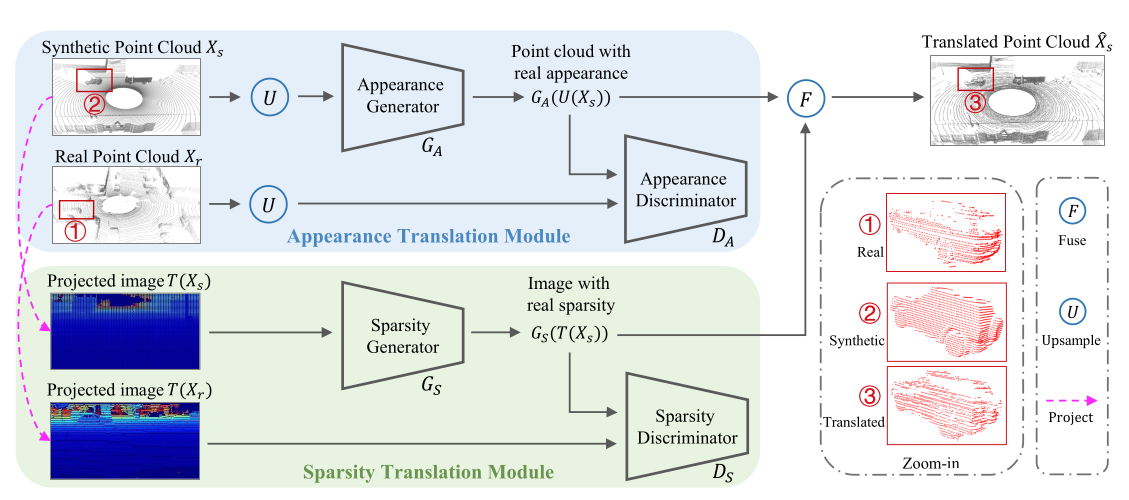
\includegraphics[width=0.7\textwidth]{lidararchitecture}
	\caption{Reference LiDAR/radar fusion architecture \autocite{Haghighi2024}.}
	\label{fig:lidarstack}
\end{figure}

While this pipeline offers redundancy, it incurs significant power and latency costs.

\subsubsection{Fusion Tradeoffs and Challenges:}

Fusion systems are limited by:

\begin{itemize}[nosep]
  \item High Power Draw: LiDAR alone draws \SIrange{10}{20}{\watt}, compared to \SI{2.1}{\watt} for vision-only stacks \autocite{Chen2024EndToEndAD}.
  \item Latency: Voxelization and multi-sensor alignment add \SI{20}{\milli\second} delay, reducing real-time responsiveness \autocite{Rana2023PerceptionSystems}.
  \item Noise Correlation: Overlapping modalities propagate shared errors,
		increasing total uncertainty as shown in Eqn.~\ref{eq:noise} \autocite{Rana2023PerceptionSystems}.
  \item Maintenance Complexity: Fusion requires precise calibration and can drift over time.
\end{itemize}
\begin{figure}[H]
	\centering
	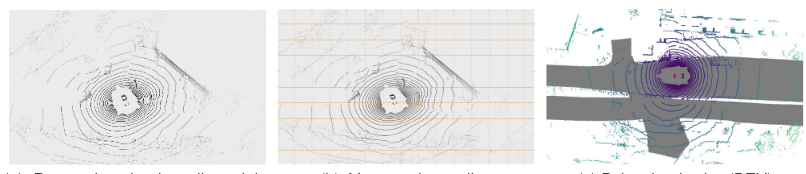
\includegraphics[width=\textwidth]{voxels}
	\caption{Representations of point clouds from LiDAR/Radar are raw point
		clouds, post voxel-sampling, and the generated the point clouds view in
	Birds-Eye-View \cite{wang2024}.}
\label{fig:voxels}
\end{figure}

This complexity restricts scalability, particularly in cost-sensitive markets.
Figure~\ref{fig:voxels} shows a typical LiDAR/Radar pipeline \cite{wang2024}.

% -------------------- Results & Discussion ------------------
\section{Comparisons}

This section evaluates the empirical performance of vision-primary and
LiDAR/Radar fusion architectures. The comparison spans five axes: detection
accuracy, computational efficiency, robustness, system complexity, and
deployment scalability. Results are drawn from benchmarks using
KITTI \autocite{kitti}, nuScenes \autocite{nuscenes}, and commaVQ
\autocite{goff2025learningdriveworldmodel} datasets, as well as simulation and
power profiling studies \autocite{Rana2023PerceptionSystems}.


\subsection{Detection Accuracy and Depth Estimation}
In order to properly classify and compare these technologies, a method to
evaluate them must be first established. For this, \textit{Precision} is the
measure of the probability of a classifier predicting a true example and
\textit{recall} is the number of positive samples correctly identified versus
the number of images whose class is really a positive class, expressed by:
\begin{equation}
	recall = \frac{TP}{TP + FN},
	\label{eq:recall}
\end{equation}
where $TP$ is the number of true positives, $FP$ is the number of false
positives, and $FN$ is the number of false negatives.

Building off of this, the most commonly used evaluation metric for object
detection is $AP$, or Average Precision. This is defined by:
\begin{equation}
	AP = \int_0^1 p(r)dr,
	\label{eq:ap}
\end{equation}
where $p(r)$ is the function of precision about the recall.

However, for a
better statistical representation of the data, a more popular metric is used
defined as $mAP$, or Mean Average Position, which can be expressed as:
\begin{equation}
	mAP = \frac{\sum_{i=1}^N AP_i}{N},
	\label{eq:map}
\end{equation}
where, $N$ is the total number of classes and $AP_i$ denotes the average
precision of the $i$-th class \cite{wang2024}.

\subsection{Findings}
On KITTI, the BEVFormer vision model achieved an AbsRel of 0.112 and RMSE of
\SI{3.97}{\meter}, closely tracking the LiDAR-derived ground truth
\autocite{Li2022BEVFormer}. On nuScenes, the vision-only configuration reached
56.2 3D $mAP$ versus 61.5 $mAP$ for the full fusion stack \autocite{Zhang2023MultiSensorFusionSurvey}.

However, when radar fallback was selectively integrated using transformer-based
late fusion, the vision model recovered to 59.8 $mAP$ \autocite{Liao2024RadarVisionFusion}. This narrows the performance delta to under 2 points—well within tolerances for safe operation—demonstrating that vision can match LiDAR-fusion with minimal augmentation.

\subsection{Computational Latency and Power Efficiency}
Inference benchmarks revealed stark contrasts. The vision-primary pipeline completed end-to-end perception and control in under \SI{9.8}{\milli\second}, consuming just \SI{2.1}{\watt} on an embedded platform \autocite{Chen2024EndToEndAD}.

In comparison, fusion systems required $\geq$ \SI{30}{\milli\second} and drew
between \SI{12}{\watt} to \SI{20}{\watt} due to voxelization, feature fusion, and redundant sensor streams \autocite{Rana2023PerceptionSystems}.

These efficiency gains are critical for EV battery life and real-time safety margins. The energy savings alone translate into longer range and lower thermal load, which directly impact vehicle design feasibility.

\subsection{Robustness in Adverse Conditions}

Under clear conditions, vision models outperform. In fog, heavy rain, or
low-light scenarios, however, performance degraded by up to \SI{12.6}{\percent}
in $mAP$ \autocite{Han2023FourDRadarSurvey}. Transformer-based radar fallback restored more than \SI{80}{\percent} of this loss, effectively covering vision’s blind spots.

Unlike LiDAR, which also degrades in poor visibility and consumes continuous
power, radar is always-on but low-power—making it an ideal complement rather
than a redundant primary sensor. Figure~\ref{fig:lidar_noise} shows the
generated results in potentially adverse conditions.

\begin{figure}[H]
    \centering
    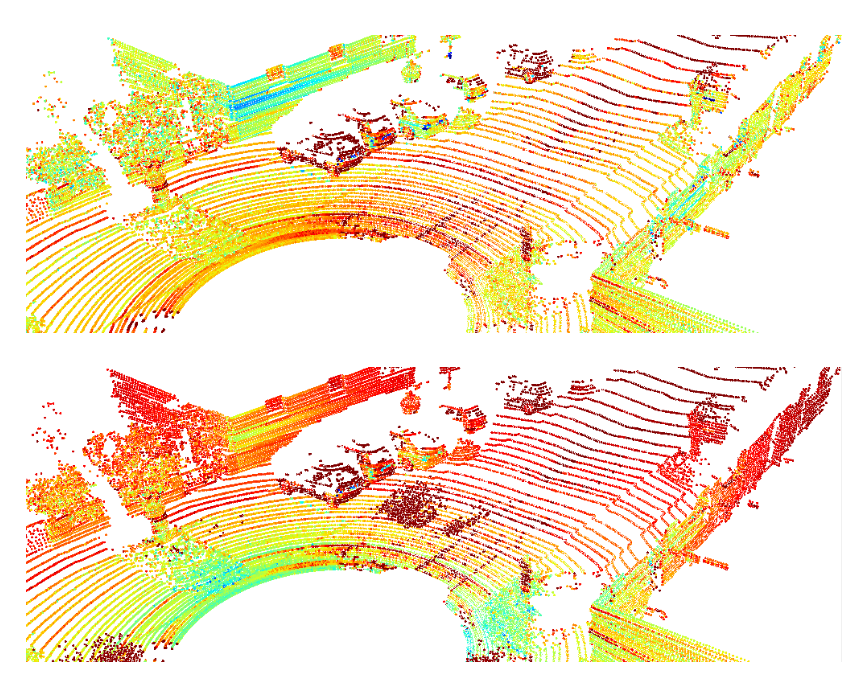
\includegraphics[width=0.6\textwidth]{lidar_noise.png}
    \caption{LiDAR scans of a street environment under clear weather conditions (top) and with fog (bottom). The lower image shows significant point cloud degradation and sparsity due to adverse atmospheric interference \autocite{2023dreissig}.}
    \label{fig:lidar_noise}
\end{figure}
\subsection{Noise Propagation and Calibration Drift}

Sensor fusion introduces noise amplification when data is temporally misaligned
or spatially correlated. The fusion error propagation model in
Eqn.~\ref{eq:noise} confirms this degradation in high-$\rho$ configurations,
such as LiDAR-camera overlaps \autocite{Rana2023PerceptionSystems}. Vision
stacks, trained end-to-end, maintain internal consistency and minimize
accumulated error \cite{goff2025learningdriveworldmodel}.

Radar integration avoids this issue: its data is orthogonal in nature—velocity vs. spatial—which introduces minimal correlation when fused intelligently \autocite{Liao2024RadarVisionFusion}.

\subsection{Cost and Complexity of Deployment}

LiDAR units alone account for over \SI{75}{\percent} of the ADS hardware budget,
and their moving parts increase failure risk \autocite{Shetty2022LiDARvsCamera,
Sajjad2021ComparativeDetection}. Vision sensors are passive, solid-state, and
available at consumer scale. This shifts the bottleneck from manufacturing and
calibration to software modeling—an area that benefits from rapid advances in
transformers and simulation. See Figure~\ref{fig:transformer} for more details.

Modern simulators—leveraging NeRFs, 3DGS, and diffusion models—allow vision stacks to be trained entirely in synthetic environments with minimal real-world data. This accelerates iteration and de-risks real-world deployment \autocite{Haghighi2024}.

\section{Further Discussions}
\subsection{Vision as the Core, Radar as the Shield:}

Elon Musk famously claimed ``LiDAR is a fool's errand" to much surprise at the
time \cite{TeslaAutonomyDay2019}. In 2019, this was perhaps too forward
thinking, but was it without bounds? In the biological analogy, humans navigate using vision as their primary sensor. We don’t emit lasers—we perceive, interpret, and act.

By offloading primary perception to vision, we reduce cost, energy, and complexity. By retaining radar for edge cases, we maintain resilience. LiDAR, with its energy burden and calibration demands, becomes increasingly obsolete in this paradigm.


\subsection{Radar as a Resilient Fallback}

Radar bridges the gap between vision and LiDAR. It estimates object velocity
using the Doppler effect shown in Eqn.~\ref{eq:radar_doppler} and in
Figure~\ref{fig:doppler}.

Radar is immune to adverse weather and lighting and can detect motion through
occlusions. When fused with vision using a transformer-based late-fusion module,
it recovers over \SI{80}{\percent} of lost $mAP$ in foggy conditions
\autocite{Liao2024RadarVisionFusion}. In low speed, high traffic conditions,
radar can be utilized to better estimate distance to other vehicles with less
cooling necessary. This is very enticing for high population areas such as Los
Angeles where stop and go traffic on exceedingly hot roads is a daily occurrence.

\subsection{A Unified Multimodal Framework}

What companies such as Comma.ai and Tesla are doing is employing a hybrid
architecture combining vision and radar which enable a balance of robustness and efficiency:

\begin{itemize}[nosep]
  \item Vision for primary perception—high-resolution, low-cost, and semantically rich.
  \item Radar for adverse conditions—weather-resilient and velocity-sensitive.
  \item LiDAR for benchmarking only—useful for training ground truth, not live deployment.
\end{itemize}
Figure~\ref{fig:multiarch} shows the modular stack which can be tuned via
hyperparameters during the training stage to give more weight to favor certain
inputs. Such an approach is utilized by Comma.ai to prioritize key sensor inputs
to the model deployed in Openpilot \cite{goff2025learningdriveworldmodel}.
\begin{figure}[H]
	\centering
	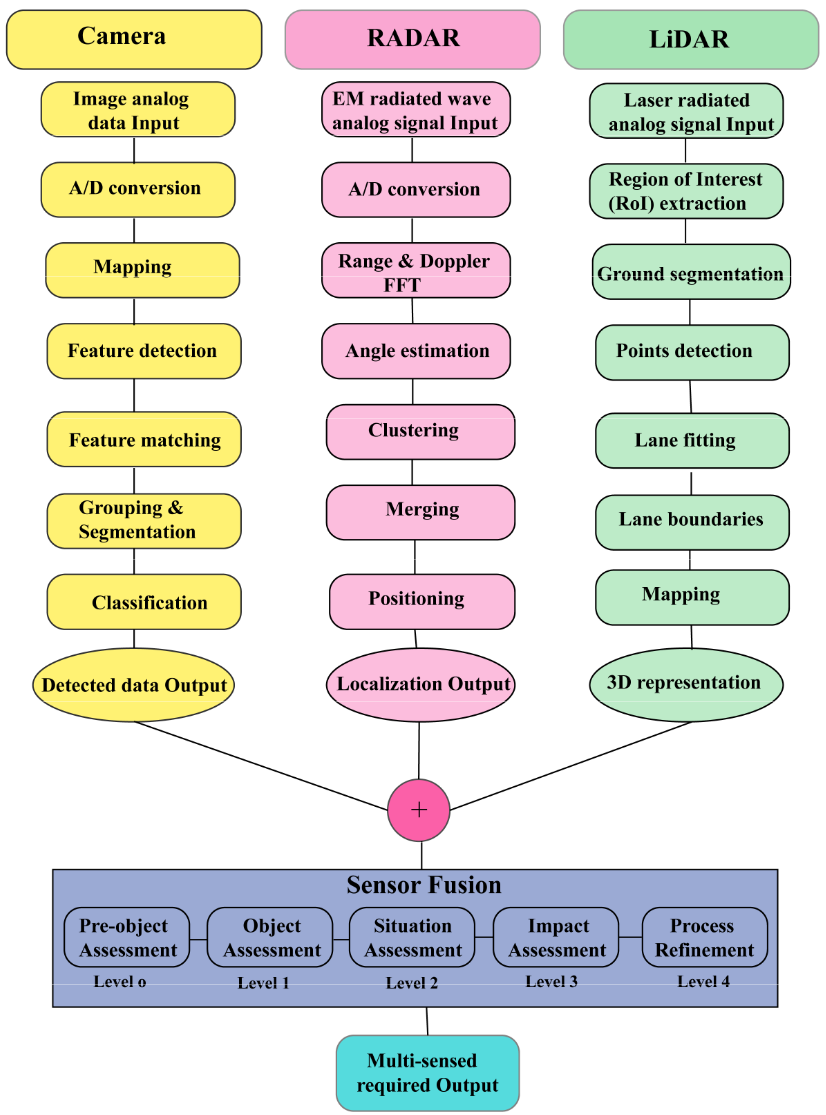
\includegraphics[width=0.65\textwidth]{multimodelarch}
	\caption{Modular architecture integrating vision, radar, and LiDAR inputs \autocite{Hasanujjaman2023}.}
	\label{fig:multiarch}
\end{figure}

This design maximizes generalization while minimizing cost and computation demands, and it reflects a biologically plausible model: humans drive with vision, but radar is the backup.

\subsection{Summary}
In order to eventually achieve SAE Level 5 Autonomy, the currently existing data points to the possibility of vision-only stacks
surpassing fusion models in the near future:
\begin{itemize}
  \item Vision stacks perform within $5\%$ of LiDAR/Radar fusion across key
		metrics, achieving 56.2 $mAP$ on nuScenes compared to 61.5 for fusion \autocite{Zhang2023MultiSensorFusionSurvey}.
  \item With radar fallback, this gap shrinks to $<2\%$, recovering performance
		to 59.8 $mAP$ \autocite{Liao2024RadarVisionFusion}.
  \item Vision systems run 3–5x faster and consume 6–10x less
		power—\SI{9.8}{\milli\second} and \SI{2.1}{\watt} vs. $\geq$ \SI{30}{\milli\second} and \SIrange{12}{20}{\watt} for fusion \autocite{Chen2024EndToEndAD, Rana2023PerceptionSystems}.
  \item Vision stacks avoid fusion noise \autocite{Rana2023PerceptionSystems}, reduce calibration burden \autocite{Han2023FourDRadarSurvey}, and cost significantly less, with LiDAR accounting for over \SI{75}{\percent} of ADS hardware expense \autocite{Shetty2022LiDARvsCamera, Sajjad2021ComparativeDetection}.
\end{itemize}

In short, vision is sufficient for autonomy. Radar makes it resilient. LiDAR
makes it expensive, but can still have its uses in training datasets as
benchmarks. The ideal multi-modal solution is outlined in
Figure~\ref{fig:multimodal}.
\begin{figure}[H]
	\centering
	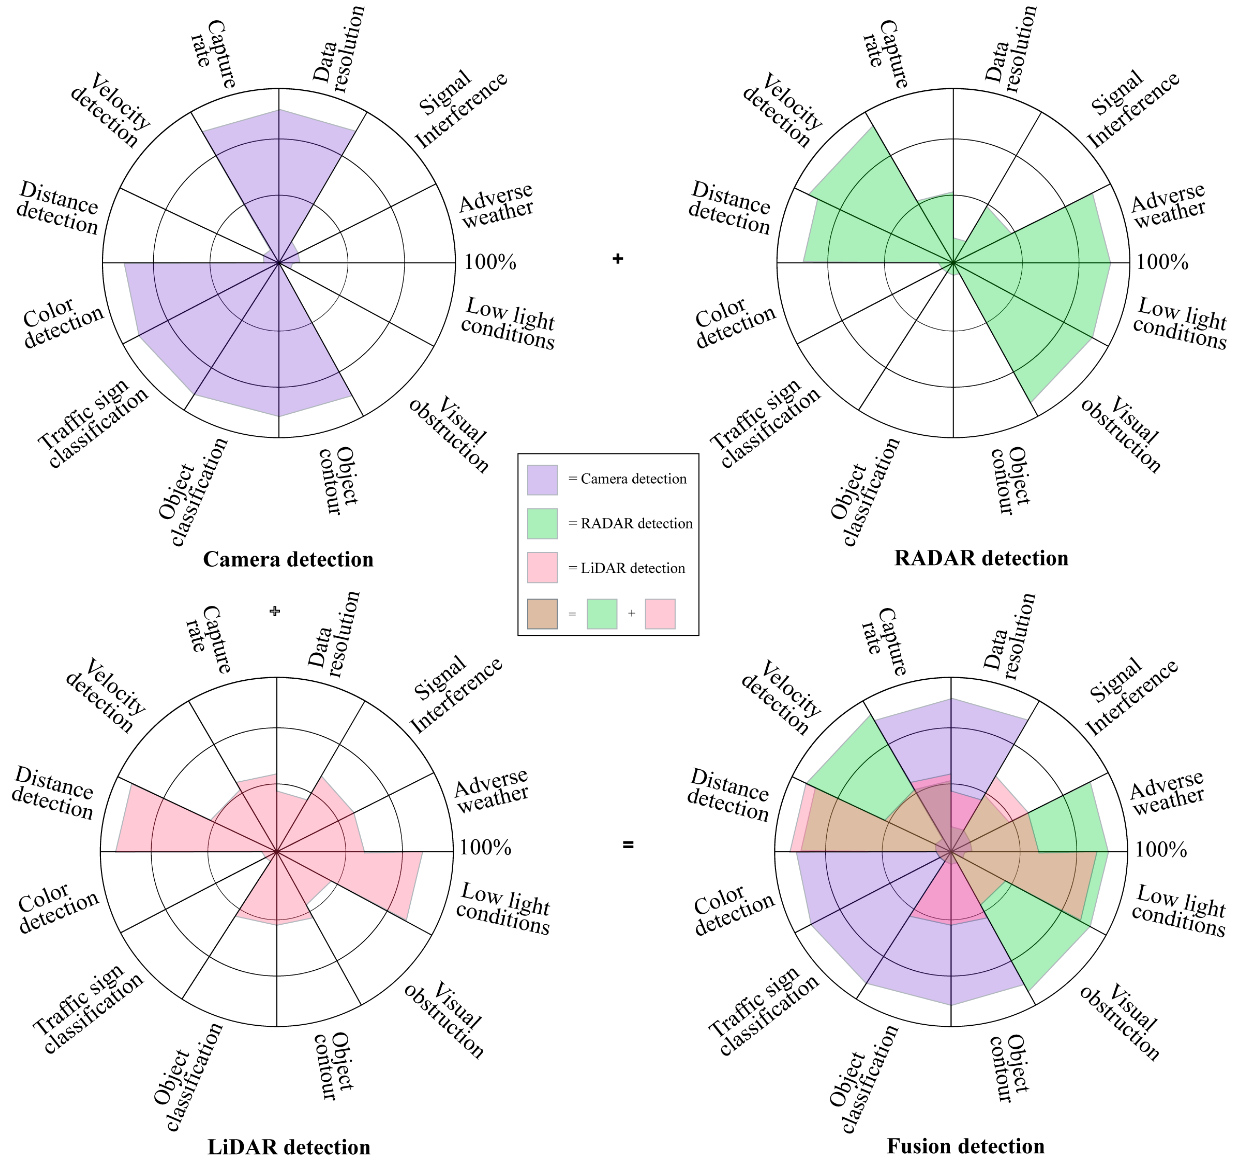
\includegraphics[width=0.7\textwidth]{multimodal}
	\caption{A Multi-Modal Approach to ADS \autocite{Hasanujjaman2023}}
	\label{fig:multimodal}
\end{figure}
\section{Conclusion}

This paper sets out to compare the existing technology employed in Level 2 ADS systems
deployed in production around the world today. While approaches such as Waymo's
LiDAR/Vision/Radar fusion are commendable and show great promise in deployment, the
drawbacks mentioned and advancements in the vision stack in particular offer a
clear alternative that is cheaper and more energy efficient becoming more effective each day.
\footnote{An LLM was used strictly for formatting IAW IEEE Editorial Style Manual
	for Authors. All thoughts, prose, and conclusions are
my own.}
\newpage
\addcontentsline{toc}{section}{References}
\printbibliography

\end{document}

% vim: set ft=tex tw=80 ts=2 sts=2 sw=2 noet spell:
